\chapter{Основы кодирования}

%code: label prefix
Далее считается, что \emph{информация} --- это упорядоченная последовательность \emph{кодовых символов}, принадлежащих конечному алфавиту. Информация является своеобразным \emph{отражением} определенного \emph{события}. Оценить количество информации просто: это число кодовых символов последовательности. Сложнее оценить сколько информации несет событие, то есть последовательности какой длины достаточно для корректного отражения события. 

Клод Шеннон в 1948 г. определил оценку количества информации, которую несет событие так:
\begin{enumerate}
    \item Количество информации $I$ есть непрерывная функция от вероятности $p$ события. 
    \item Количество информации $I_i$ одиночного $i$-го события $s_i$, $s_i\in S$ ($S$ --- множество всех событий), $i\in[1,n]$ ($n$ --- количество различных событий в $S$), происходящего с вероятностью  $p_i$, имеет положительное значение $I_i\geq 0$;$I_i=I(p_i)$. Причем  $\sum_{i=1}^n p_i=1$.
    \item Совместное количество информации $I_{ij}$ двух независимых событий $s_i$,$s_j$ с совместной вероятностью $p_{ij}=p_i\cdot p_j$, равна сумме их количеств их информаций $I_{ij}=I_i+I_j$; $I(p_i\cdot p_j )=I(p_i )+I(p_j)$.
\end{enumerate}

\begin{exampl}
    Количество воспринимаемой информации влияет на эмоциональное состояние человека и постулаты Шеннона легко проверить на себе.
    
    Согласно Шеннону, количество информации зависит от вероятности наступления события. Сравните свои эмоции от двух событий: <<Жучка укусила Иванова>> и <<Иванов укусил Жучку>>. Первое событие, хоть собака и друг человека, будничное, а вот второе вызывает улыбку --- сенсация! Вероятность первого события весьма велика, вероятность второго близка к нулю. Первое событие несет мало информации, а второе несет большое её количество, отсюда и эмоции.

    В то же время, если мы на следующий день услышим, что после Иванова Жучку укусил еще и Петров, то внутренне мы будем готовы к тому, что на третий день Жучку укусит и Сидоров --- только ленивый не кусает Жучку! Хотя по правилам теории вероятности, с точки зрения обывателя, который не в курсе отношений Жучки с людьми, вероятность того, что Жучку укусит Иванов также мала, как и вероятность быть покусанной Петровым, и равна $p$. Вероятность, того, что Жучка будет покусана обоими, равна произведению вероятностей этих событий: $p^2$ --- это практически невероятно, так как $p^2$ много меньше $p$ и следует ожидать большой сенсации. Но! Никто (разве что Жучка) не падает в обморок от совместных действий Иванова и Петрова, так как количество информации, которое несет данное событие, есть лишь сумма количеств информаций для каждого факта оскорбления действием Жучки в отдельности.
    \qed
\end{exampl}

Постулатам Клода Шеннона удовлетворяет функция:
\begin{equation}
    \label{eq:code:shannon}
    I(p)=-\log_m p,
\end{equation}
где $p$ --- вероятность события, а $m$ количество кодовых символов в алфавите. При этом $m$ определяет единицы измерения информации. Например:
\begin{itemize}
    \item $m=2$: $[I]$ --- бит;
    \item $m=e$: $[I]$ --- нат;
    \item $m=3$: $[I]$ --- трит;
    \item $m=10$: $[I]$ --- дит.
\end{itemize}

Процесс сопоставления событиям информационных цепочек называется \emph{кодированием}.

Изложение  математических основ кодирования можно найти, например, в \cite{bib:novic:discrmathprogrammer,bib:yablonsky:discreteintro}. По основам теории информации можно рекомендовать книгу \cite{bib:panin:informationTheory}. Основы кодирования подробно изложены в \cite{bib:verner:codingBase}. Краткая теория приведена ниже.


\section{Назначение и формальное определение кодирования}

Можно выделить следующие основные назначения кодирования:
\begin{itemize}
    \item принципиальная возможность описания мира с помощью \emph{символов} конечного алфавита;
    \item устранение избыточности информации, её сжатие, и как следствие экономия памяти и снижение нагрузки на каналы передачи информации;
    \item защита информации (точнее защита таких свойств информации как: конфиденциальность, целостность, принадлежность, и т.д.).
\end{itemize}

Рассмотрим классическую задачу <<о картах>>:
\begin{exampl}
    \label{exampl:code:cards}
    Задача о картах. Имеется колода из восьми карт. По две карты (допустим, туз и двойка) каждой масти. Профессор вытягивает наугад карту и готов честно давать ответы да/нет на любые задаваемые вопросы. Нужно минимальным количеством вопросов угадать вытащенную карту.
\end{exampl}
\begin{proof}[Решение]
    Можно решить задачу задавая вопросы о конкретной карте. Тогда можно угадать карту с первого вопроса, но вероятность тому весьма мала. В худшем же случае, очевидно, потребуется семь вопросов.
    
    Более <<тонкое>> решение: каждым вопросом сокращать неопределенность вдвое. Например, ответ на первый вопрос о цвете масти разделит нам исходную колоду на две равные части по четыре карты. Вопрос о конкретной масти оставит нам две карты. И вопрос о достоинстве карты будет последним. 
    
    На рисунке \ref{fig:code:cards} ответам <<да>> соответствует символ $0$, а <<нет>> --- $1$. Продвигаясь от вершины дерева до конкретной карты поставим ей в соответствие получаемую цепочку символов. Эта цепочка символов и будет являться \emph{кодом} карты.
    
    \begin{figure}
        \centering
        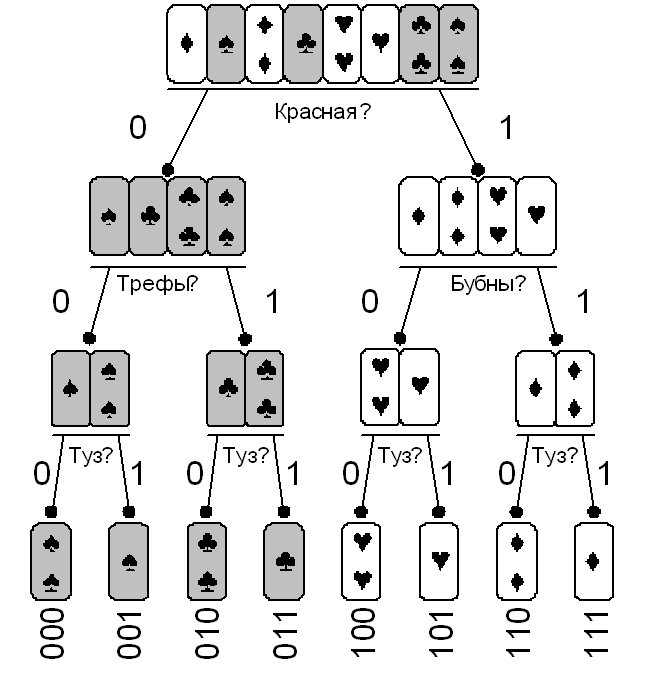
\includegraphics[width=0.47\textwidth]{fig/cards}
        \caption{Решение задачи о картах}
        \label{fig:code:cards}
    \end{figure}
    
    Теперь, договорившись с профессором о способе кодирования, можно попросить его так же честно сообщать \emph{код} вытащенной карты. И если он передал вам записанную на бумажке цепочку символов $011$, вы без труда догадаетесь, что из колоды был изъят туз треф.
\end{proof}

Полученную в процессе кодирования цепочку-информацию далее можно преобразовать в \emph{сигнал} и передавать по каналам связи. Так, например, непосредственный контакт с профессором из примера \ref{exampl:code:cards} больше не нужен: информация о карте может быть передана миганием фонарика, стуком, морзянкой по радио и т.д.

Не нужно забывать, что кроме \emph{бита} существуют и другие единицы измерения информации.
\begin{exampl}
    \label{exampl:code:femida}
    Задача о биллиардных шарах. Имеется восемь биллиардных шаров с номерами $1$-$8$ соответственно. Все шары одинаковой массы, кроме одного, который тяжелее остальных. Имеются весы Фемиды (чашечные). Какое количество взвешиваний вам потребуется, чтобы определить номер тяжелого шара?
\end{exampl}
\begin{proof}[Решение] 
    Весы Фемиды выдают информацию тритами, поэтому вам потребуется всего два вопроса. Коды шаров будут состоять из двух символов (см. рис. \ref{fig:code:femida}).
    \begin{figure}
        \centering
        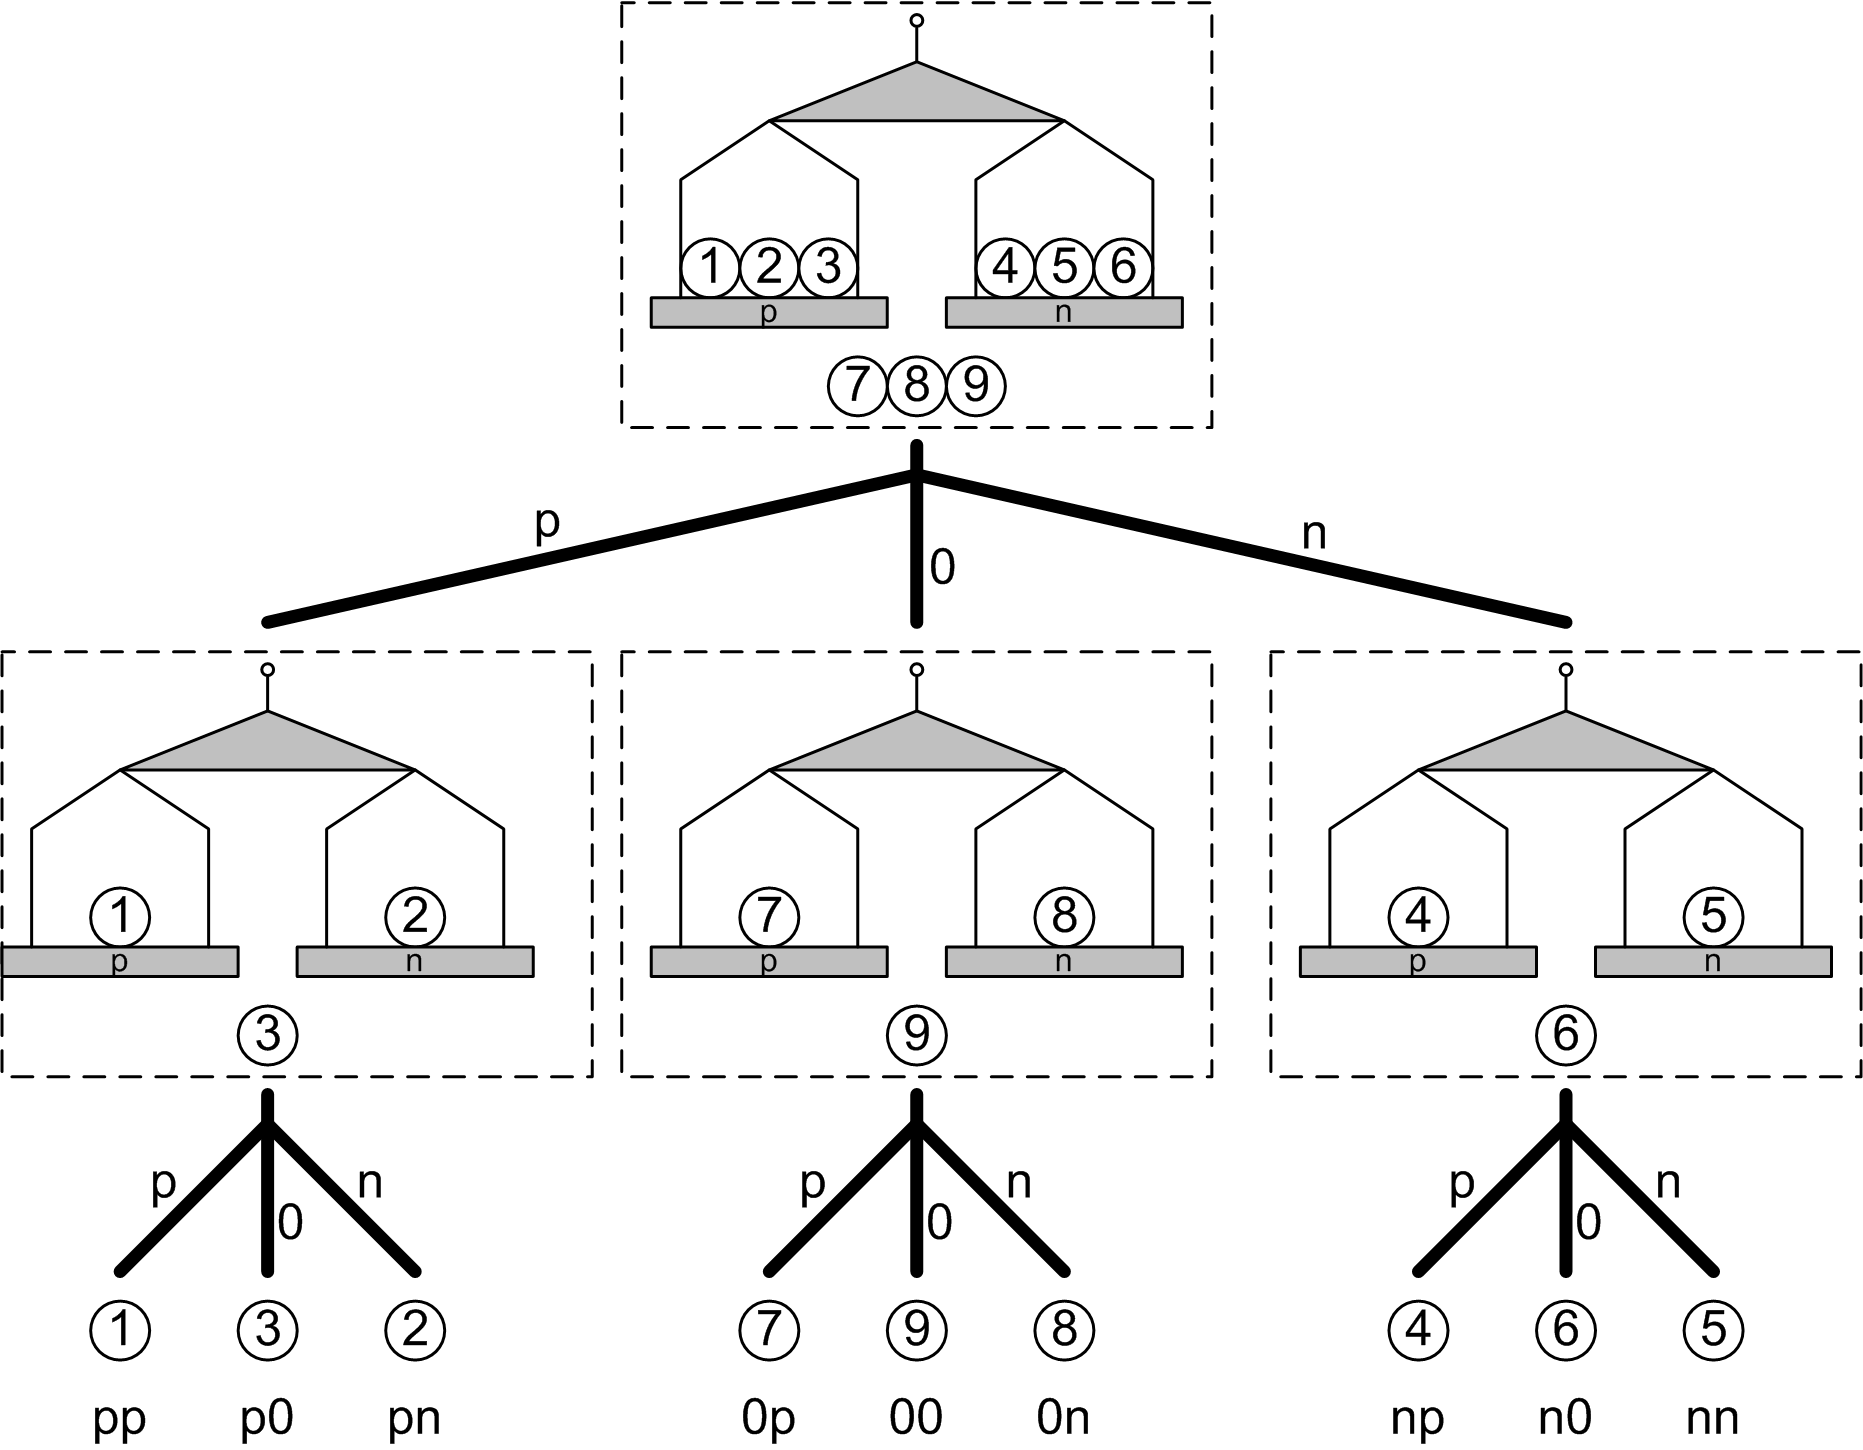
\includegraphics[width=0.47\textwidth]{fig/femida}
        \caption{Решение задачи о картах}
        \label{fig:code:femida}
    \end{figure}    
\end{proof}

Формально кодирование можно определить так. Имеется множество (алфавит) \emph{событий} 
\[
    S=\{s_1,\ldots,s_n\},
\] где $s_i$ --- буква алфавита событий (событие), $n$ --- количество событий (букв) алфавита $S$.

Алфавит \emph{кодовых символов}:
\[
    A=\{a_1,\ldots,a_m\},
\] где $a_i$ --- буква кодового алфавита (символ), а $m$ --- количество смволов в $A$. 

Требуется задать соответствие (схему, таблицу кодов) $\delta$ между событием $s_i$ и \emph{кодовым словом} $\omega_i=a_{i_1}\cdots a_{i_k}$:
\[
    \delta=\{ s_1\mapsto\omega_1, \ldots, s_n\mapsto\omega_n\}.
\]

Причем слово $\varsigma_j$, состоящее из букв алфавита $S$
\[
    \varsigma_j=s_{j_1}\cdots s_{j_t}
\]
будет кодироваться символами кодового алфавита как
\[
    \varsigma_j=\omega_{j_1} \cdots \omega_{j_t}.
\]
Множество кодовых слов $\omega_i$, соответствующих $s_i$ называется множеством \emph{элементарных кодов}:
\[
\Omega=\{\omega_1,\ldots,\omega_n\},
\]

\begin{exampl}
    Для кодирования \emph{букв} из множества $S=\{A,B,C,D,E,F,G,H\}$ с помощью \emph{слов} алфавита $A=\{0,1\}$ применяется следующее соответствие:
    \[
    \begin{split}
        \delta=\{ 
            A \mapsto 0,
            B \mapsto 1,
            C \mapsto 10,
            D \mapsto 11,
            E \mapsto 100,\\
            F \mapsto 101,
            G \mapsto 110,
            H \mapsto 111
        \}
    \end{split}
    \]

    Как видно, такое кодирование однозначно, но не взаимо однозначно. Слову $ABBA$ однозначно соответствует $0110$, а вот цепочке $0110$ соответствуют еще и
    \[AG\xrightarrow{\delta} 0110 \xleftarrow{\delta} ADA.\]

    Взаимно однозначный вариант кодирования может быть следующим:
    \[
        \begin{split}
            \delta=\{ 
                A \mapsto 000,
                B \mapsto 001,
                C \mapsto 010,
                D \mapsto 011,
                E \mapsto 100,\\
                F \mapsto 101,
                G \mapsto 110,
                H \mapsto 111
            \}
        \end{split}
    \]

    Теперь
    \[ABBA\xrightarrow{\delta} 000001001000\]
    декодируется однозначно.
    \qed
\end{exampl}

Таблица кодов $\delta$ является \emph{разделимой}, если любое слово $\varsigma_j$, составленное из элементарных кодов $\omega_i$ единственным образом разлагается на элементарные коды. При этом в таблице кодов не допускается, чтобы одному и тому же элементарному коду соответствовали различные буквы алфавита событий $s_i$.  Разделимая схема допускает \emph{декодирование}.

Важным частным случаем разделимых схем являются \emph{префиксные} схемы. Схема называется \emph{префиксной}, если ни один элементарный код $\omega_i$  из множества $\Omega$ не является префиксом другого кода из того же множества. \emph{Префиксом}, началом или приставкой слова $\omega$ называется слово $\omega_1$, если $\omega=\omega_1 \omega_2$. \emph{Постфиксом} или окончанием называется, соответственно, слово $\omega_2$. Коды, полученные на основе кодирующего дерева, см. например, рис. \ref{fig:code:cards}, очевидно, являются префиксными.

Наиболее простым вариантом кодирования является \emph{равномерное} кодирование, когда все элементарные коды одной длины. В этом случае требуется оценить длину цепочки кода, если количество кодируемых событий равняется $n$, а количество кодовых букв равняется $m$. Цепочкой из одного кодового символа можно закодировать $m$ событий, из двух --- $m^2$ и т.д. В общем случае из цепочкой из $I$ символов можно закодировать $m^I$ событий. Следовательно
\[
    I(n)=\lceil\log_m(n)\rceil,
\]
где $\lceil X \rceil$ --- наименьшее целое, большее или равное $X$.

Эту же оценку можно получить на основе постулатов Шеннона, предположив, что события равновероятны (т.е. вероятность любого события $p=\frac{1}{n}$). Тогда, в соответствии с формальным определением количества информации (см. формулу \eqref{eq:code:shannon}) для равномерного кодирования потребуется взять кодовые слова следующей длины:
\[
    I(n)=\lceil -\log_m\left(\frac{1}{n}\right)\rceil=\lceil \log_m(n) \rceil.
\]

Для приведенного примера с картами (пример \ref{exampl:code:cards}) длина кодов составляет $I(8)=\lceil \log_2(8) \rceil=3$ бита, а для примера (пример \ref{exampl:code:femida}) с весами Фемиды $I(8)=\lceil \log_3(8) \rceil=2$ трита.

\begin{exampl}
    В соревновании учавствуют $17$ спортсменов. Для регистрации пересечения финишной черты каждому спортсмену выдается радио-брелок. В момент пересечения финишной черты спортсменом, брелок передает двоичный код для идентификации спортсмена. Все брелки передают код одинаковой длины. Какое минимально необходиоме количество бит в общем случае должен передать брелок?
\end{exampl}
\begin{proof}[Решение] $\lceil \log_2(17)\rceil = 5$.
\end{proof}

В ряде случаев в процессе кодирования имеются знания о вероятности возникновения тех или иных событий. Если это так, то можно использовать методики оптимального кодирования для экономии памяти (или снижения нагрузки на каналы передачи данных).


\section{Оптимальное кодирование}

\emph{Источнику событий} после кодирования соответствует \emph{источник информации}, то есть источник, выдающий коды событий. Оценку информативности источника событий дает величина, называемая \emph{энтропией}:
\begin{equation}
    \label{eq:code:entrophyS}
    E=-\sum_{i=1}^n {p_i\cdot\log_m p_i},
\end{equation}
где $p_i$ --- вероятность $i$-го события $s_i\in S$ на выходе источника событий, $m$ --- количество информационных символов, используемых для кодирования, $n$ --- количество событий.

Так как вероятности появления кодов событий останутся прежними, то энтропия источника информации $E'$ будет равна
\begin{equation}
    \label{eq:code:entrophyI}
    E'=\sum_{i=1}^n {p_i\cdot I_i},
\end{equation}
где $I_i$ --- длина кода $\omega_i$ для $i$-го события .

Энтропия источника информации всегда больше энтропии отражаемого источника событий. Задача оптимального кодирования максимально приблизить энтропию источника информации к источнику событий.
\begin{exampl}
    Пусть имеется источник событий $s_i$, о вероятности появления которых на его выходе известно следующее:
    
    \begin{tabular}{|l|c|c|c|c|}
        \hline
        Событие $s_i$                   &А      &Б      &В      &Г   \\ \hline
        Вероятность $p_i$ события $s_i$ &0.5    &0.3    &0.1    &0.1 \\ \hline
    \end{tabular}
    
    Энтропия источника событий (формула \ref{eq:code:entrophyS}) составляет
    \[
        \begin{split}
            E=-(0.5\cdot\log_2 0.5+0.3\cdot\log_2 0.3+0.1\cdot log_2 0.1+0.1\cdot log_2 0.1)\approx \\
            \approx(0.5+0.521089678+0.332192809+0.332192809)\approx 1.685475297\text{\,бит}.
        \end{split}
    \]
    
    Для равномерного кодирования битами может быть получен такой вариант:

    \begin{tabular}{|l||c|c|c|c|}
        \hline
        Событие $s_i$                   &А      &Б      &В      &Г   \\ \hline
        Вероятность $p_i$ события $s_i$ &0.5    &0.3    &0.1    &0.1 \\ \hline
        Код события $\omega_i$          &00     &01     &10     &11  \\ \hline
    \end{tabular}
    
    Энтропия данного источника информации составит (формула \ref{eq:code:entrophyI})
    \[
        E'=(0.5\cdot 2+0.3\cdot 2+0.1\cdot 2+0.1\cdot 2)=2 \text{\,бита}.
    \]
    
    Видно, что энтропия источника информации значительно больше. Можно ли её уменьшить, приблизить к энтропии источника событий? Очевидно, что если кодировать символы с большей вероятностью появления кодом с меньшей длиной, то результаты должны получиться лучше. Попробуем следующую схему:
    
    \begin{tabular}{|l||c|c|c|c|}
        \hline
        Событие $s_i$                   &А      &Б      &В      &Г   \\ \hline
        Вероятность $p_i$ события $s_i$ &0.5    &0.3    &0.1    &0.1 \\ \hline
        Код события $\omega_i$          &0      &10     &110    &111 \\ \hline
    \end{tabular}
    
    Так же как и предыдущая, эта схема префиксная и разделимая, но неравномерная. Энтропия источника информации теперь составляет
    \[
        E'=(0.5\cdot 1+0.3\cdot 2+0.1\cdot 3+0.1\cdot 3)=1.7\text{\,бита}.
    \]
    Результаты много лучше! Так, если запустить источник информации на выдачу, например, $100$ кодов событий  то первый вариант кодирования выдаст нам цепочку длины примерно $200$, а второй примерно $170$ бит. Существенная экономия при том же качестве.
    \qed
\end{exampl}

Далее рассматриваются два алгоритма оптимального кодирования источника событий: алгоритм Хаффмана и алгоритм Фано. 
\paragraph{Алгоритм Хаффмана для $m=2$ (двоичное кодирование)}
\begin{enumerate}
    \item\label{enum:code:haffman2Sort} События сортируются по убыванию вероятности.
    
    \item\label{enum:code:haffman2Step} Два события с минимальными вероятностями объединяются в одно составное событие, которое имеет вероятность, равную сумме вероятностей исходных событий. При этом одно из исходных событий помечается кодовым символом $0$, а второе --- символом $1$. Исходные события исключаются из множества событий, вместо них остается одно составное. 
    
    \item Шаги \ref{enum:code:haffman2Sort} и \ref{enum:code:haffman2Step} последовательно повторяются до тех пор, пока все события не склеятся в единственное составное событие (корень), вероятность которого, очевидно, равна $1$. После этого кодовое слово $\omega_i$ для исходного события $s_i$ есть цепочка из кодовых символов, которыми помечены все составные события от  корня до $s_i$.
\end{enumerate}

\begin{exampl} Задача. С помощью алгоритма Хаффмана закодировать следующий источник событий.

    \begin{tabular}{|l||c|c|c|c|c|}
        \hline
        Событие $s_i$                   &А      &Б      &В      &Г      &Д      \\ \hline
        Вероятность $p_i$ события $s_i$ &0.5    &0.125  &0.125  &0.125  &0.125  \\ \hline
    \end{tabular}
\end{exampl}
\begin{proof}[Решение]
    Ход выполнения алгоритма Хаффмана отражен на рисунке \ref{fig:code:haffman2Ex}. После сортировки событий по убыванию вероятности видно, что вариантов для склеивания несколько. Произвольно выбираются два события с наименьшими вероятностями:Г и Д(энтропия от этого выбора не изменится). События Г и Д склеиваются в событие ГД с вероятностью $0.25$. Г помечается кодовым символом $0$, а Д --- $1$. Теперь множества событий выглядит так: \{А,Б,В,ГД\}. Наименьшую вероятность имеют события Б и В, которые и склеиваются в событие БВ с вероятностью $0.25$. Событие Б помечено символом $0$, а В --- $1$. Множество событий имеет вид {А,БВ,ГД}. Наименьшую вероятность имеют события БВ и ГД, которые и склеиваются в событие БВГД с вероятностью $0.5$. Событие БВ отмечено символом $0$, событие ГД символом $1$. Множество событий теперь имеет вид {А,БВГД}. Отмечая событие А символом $0$, а событие БВГД символом $1$, приходим к единственному событию в множестве событий {АБВГД} с вероятностью $1$.
    \begin{figure}
        \centering
        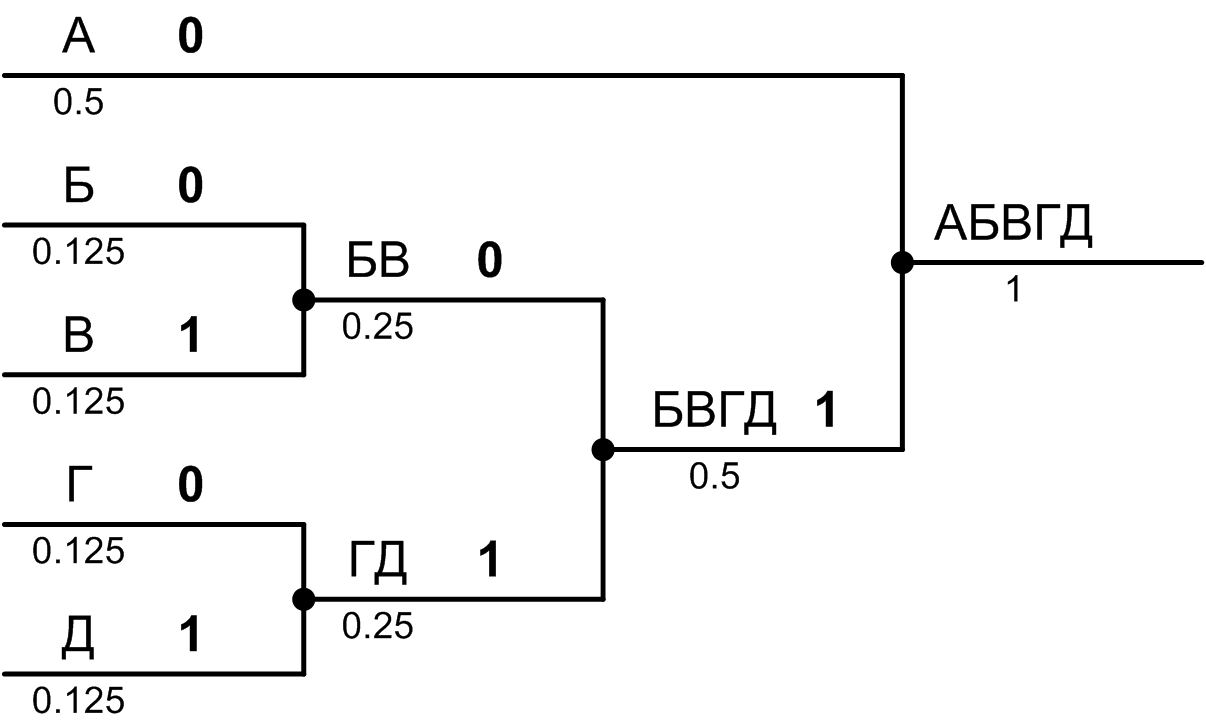
\includegraphics[width=0.6\textwidth]{fig/haffman2Ex}
        \caption{Кодирование источника по Хаффману}
        \label{fig:code:haffman2Ex}
    \end{figure} 
    Далее продвигаясь от корня (события АБВГД) до события исходного множества формируются кодовые слова $\omega_i$ из символов, которыми помечены промежуточные события на этом пути:
    \begin{tabular}{|l||c|c|c|c|c|}
        \hline
        Событие $s_i$                   &А      &Б      &В      &Г      &Д      \\ \hline
        Вероятность $p_i$ события $s_i$ &0.5    &0.125  &0.125  &0.125  &0.125  \\ \hline
        Код события $\omega_i$          &0      &100    &101    &110    &111    \\ \hline
    \end{tabular}
    
    Автоматически получен префиксный код. Попробуйте декодировать цепочку $10001101110111$.
\end{proof}

\paragraph{Алгоритм Фано для $m=2$}
\begin{itemize}
    \item[] На входе алгоритма имеется исходный массив событий, отсортированный в порядке убывания соответствующих им вероятностей (предполагается, что событий больше, чем $m$, иначе кодирование тривиально --- по одному символу на событие). Далее исходный массив разбивается на две части, так, чтобы разница сумм вероятностей событий каждой части была минимальна. Первый кодовый символ элементарного кода $\omega_i$ для каждого события $s_i$ находится так: для всех событий левой части разбитого массива первый кодовый символ будет $0$, а для всех событий правой части --- $1$. Второй и последующие кодовые символы определяется так: каждая часть разбитого исходного массива, в которой более одного события, становится исходным массивом, а разбиение с нахождением кодового символа для входящих в нее событий выполняется так же как для исходного массива.
\end{itemize}

\begin{exampl} Задача. С помощью алгоритма Фано закодировать следующий источник событий.

    \begin{tabular}{|l||c|c|c|c|c|c|c|c|}
        \hline
        $s_i$   &А      &Б      &В      &Г      &Д      &Е      &Ж      \\ \hline
        $p_i$   &0.135  &0.24   &0.25   &0.125  &0.0635 &0.124  &0.0625 \\ \hline
    \end{tabular}
\end{exampl}
\begin{proof}[Решение]
    Выполнение алгоритма Фано приводится в таблице \ref{table:code:fano}.
    \begin{table}
        \centering
        \begin{tabular}{|c|c||c|c|c|c|}
            \hline\hline
            $s_i$   &$p_i$  &\multicolumn{4}{c|}{$\omega_i$}\\ \hline\hline
            В       &0.25   &0&0&\multicolumn{2}{c|}{}      \\ \cline{4-4}
            Б       &0.24   &0&1&\multicolumn{2}{c|}{}      \\ \cline{3-5}
            А       &0.135  &1&0&0&                         \\ \cline{5-5}
            Г       &0.125  &1&0&1&                         \\ \cline{4-5}
            Е       &0.124  &1&1&0&                         \\ \cline{5-6}
            Д       &0.0635 &1&1&1&0                        \\ \cline{6-6}
            Ж       &0.0625 &1&1&1&1                        \\ \hline            
        \end{tabular}
        \caption{Выполнение алгоритма Фано}
        \label{table:code:fano}
    \end{table}
    
    На первом шаге найдем минимальную разницу сумм вероятностей среди вариантов разбиения на части: В:БАГЕДЖ=$|0.25-0.75|=0.5$; ВБ:АГЕДЖ=$|0.49-0.51|=0$.02; ВБА:ГЕДЖ=$|0.625-0.375|=0.25$; и т.д. очевидно, минимум это вариант ВБ:АГЕДЖ. Первый кодовый символ для событий части ВБ --- 0, для остальных событий части АГЕДЖ  --- 1. Имеем две части, для каждой из которых повторяется тот же алгоритм. Продолжим с частью АГЕДЖ, как с более интересной: А:ГЕДЖ=$|0.135-0.375|=0.24$; АГ:ЕДЖ=$|0.26-0.25|=0.01$; АГЕ:ДЖ=$|0.384-0.126|=0.258$; и т.д. минимум --- вариант АГ:ЕДЖ. Второй кодовый символ для событий АГ --- $0$, для событий ЕДЖ --- $1$. Для каждой части АГ и ЕДЖ повторяется тот же алгоритм. Например, для части АГ имеется единственный вариант разбиения А:Г и третий кодовый символ для А --- $0$, а для Г --- $1$. Так ни в одной части количество событий не превосходит единицы и делить уже нечего, то кодовые слова для событий А и Г определены. И так для всех получаемых частей.
\end{proof}


\section{Кодирование с целью сжатия информации}

Следует выделить различия между между \emph{оптимальным кодированием} и \emph{кодированием с целью сжатия}? Оптимальное кодирование ставит себе в задачу сопоставить источнику событий минимальное количество адекватной ему информации. Кодирование с целью сжатия ставит себе в задачу уменьшить количество информации, не теряя (или оставаясь в допустимых рамках) при этом свойство адекватности. Кодирование с целью сжатия будем далее называть просто \emph{сжатие}. В случае сжатия события $s_i$ уже представляют собой слова в алфавите $A$. То есть информация \emph{перекодируется} в том же алфавите $A$.

Выделяют два больших класса алгоритмов сжатия информации: сжатие с потерями и без потерь. Теряется, данном случае, конечно, адекватность отражения. При сжатии без потерь из сжатой информации можно восстановить исходную информацию в точности такую же, как до сжатия. При сжатии с потерями восстановленная информация будет отличаться от исходной. Ярким примером сжатия с потерями является сжатие изображений: используя определенные особенности восприятия цвета человеком, такие алгоритмы отбрасывают <<лишнюю>> информацию. Потеря адекватности отражаемому объекту в этом случае значительная, но для человека-потребителя эти потери адекватности незаметны.

Часто алгоритмы сжатия весьма специфичны и учитывают особенности отражаемого источника событий. Одним из важнейших таких источников в жизни человека является речь. Письмо --- способ кодирования речи с помощью символов конечного алфавита --- азбуки. На основе, например, русского алфавита можно построить бесконечное количество слов, но в реальной жизни словарный запас редко превышает сотню тысяч слов. На практике для универсального представления текста байтами кодируются буквы, цифры, знаки препинания, пробелы и т.д., но если мы знаем, что кодируется именно осмысленный текст (содержащий осмысленные слова), то можно сильно сэкономить, кодируя в качестве сообщений $s_i$ не буквы, а слова. Такие методы сжатия называются \emph{словарными}. 

Впрочем, словарные методы могут использоваться не только для кодирования текста, но для произвольных информационных цепочек. Причем словарь может строиться динамически и совершенно не учитывать смысловой нагрузки слов в словаре.

Далее будет рассмотрен алгоритм Лемпела-Зива, относящийся к группе словарных. В основе алгоритма Лемпела-Зива лежит идея \emph{адаптивного} сжатия: за один проход по цепочке одновременно строится и словарь и код, причем словарь не хранится, так как при декодировании он динамически восстанавливается.

\paragraph{Алгоритм Лемпела-Зива}
\begin{itemize}
	\item Кодирование
	\begin{enumerate}
		\item В словарь нулевым элементом помещается пустая цепочка $\varepsilon$. Пустое слово $\varepsilon$ не содержит букв и для любого слова $\omega$ справедливо $\omega=\varepsilon\omega=\omega\varepsilon$.
        
        \item\label{enum:code:lzWord} От исходной цепочки $t$ отделяется слово $\omega a$, где $\omega$ --- максимально длинное слово из словаря, $a$ --- расширяющая буква. Т.е. $t=\omega at'$.
        
        \item\label{enum:code:lzDict} В конец словаря добавляется новое слово $\omega a$. К коду c добавляется пара $\langle i_{\omega},a\rangle$, где $i_{\omega}$ --- индекс слова $\omega$ в словаре. От исходного текста отделяется слово $\omega a$: $t=t'$.
        
        \item Пункты \ref{enum:code:lzWord}-\ref{enum:code:lzDict} последовательно повторяются до тех пор, пока в тексте $t$ остается хоть одна буква.
	\end{enumerate}
    В результате получается код $c=\langle i_1,a_1\rangle\cdots\langle i_n,a_n\rangle$.
    
	\item Декодирование
    \begin{enumerate}
        \item В словарь нулевым элементом помещается пустая цепочка $\varepsilon$. Текст $t$ не содержит букв: $t=\varepsilon$.
        
        \item\label{enum:code:lzDecode} От исходного кода c отделяется пара $\langle i,a\rangle$, в словарь добавляется слово $\omega_i a$, где $\omega_i$ --- $i$-е слово из словаря (словарь восстанавливается так же, как и формируется!). Восстанавливается текст $t=t\omega_i a$.
        
        \item Пункт \ref{enum:code:lzDecode} последовательно повторяется до тех пор, пока в коде $c$ остается хоть одна пара.
    \end{enumerate}
\end{itemize}

Нужно отметить, что данный алгоритм хорошо сжимает тексты большого объема, в которых так или иначе будут присутствовать одинаковые и достаточно длинные слова. В следующем примере такие вхождения были созданы искусственно.

\begin{exampl} 
    Задача. Сжать текст <<АБАКАНКАНКАНКИАНКИН>>. Оценить выигрыш от сжатия. Восстановить текст из кода.
\end{exampl}
\begin{proof}[Решение]
    Процесс кодирования отражен в таблице \ref{t:code:lzEncodeEx}. Процесс декодирования в таблице \ref{t:code:lzDecodeEx}. Если предположить, что символы текста кодируются байтом, а каждая пара кода $\langle i,a \rangle$ двумя байтами (байт на индекс $i$, второй на букву $a$), то в данном случае объем текста $19$ байт, а кода --- $16$. Коэффициент сжатия $\frac{19}{16}$.
    \begin{table}
        \centering
        \begin{tabular}[c]{|l|l|l|l|}
            \hline\hline
            $i$ & $t$                                            & $\omega a$                         & $c=\langle i_\omega,a\rangle$ \\ 
            \hline\hline
              &                                                  & $0\mapsto\varepsilon $   & \\ \hline
            1 &	$\varepsilon\text{\textbf{А}БАКАНКАНКАНКИАНКИН}$ & $1\mapsto\text{A}    $   & $\langle\text{0,А}\rangle$ \\ \hline
            2 &	$\varepsilon\text{\textbf{Б}АКАНКАНКАНКИАНКИН} $ & $2\mapsto\text{Б}    $   & $\langle\text{0,Б}\rangle$ \\ \hline
            3 &	$           \text{\textbf{АК}АНКАНКАНКИАНКИН}  $ & $3\mapsto\text{АК}   $   & $\langle\text{1,К}\rangle$ \\ \hline
            4 &	$           \text{\textbf{АН}КАНКАНКИАНКИН}    $ & $4\mapsto\text{АН}   $   & $\langle\text{1,Н}\rangle$ \\ \hline
            5 &	$\varepsilon\text{\textbf{К}АНКАНКИАНКИН}      $ & $5\mapsto\text{К}    $   & $\langle\text{0,К}\rangle$ \\ \hline
            6 &	$           \text{\textbf{АНК}АНКИАНКИН}       $ & $6\mapsto\text{АНК}  $   & $\langle\text{4,К}\rangle$ \\ \hline
            7 &	$           \text{\textbf{АНКИ}АНКИН}          $ & $7\mapsto\text{АНКИ} $   & $\langle\text{6,И}\rangle$ \\ \hline
            8 &	$           \text{\textbf{АНКИН}}              $ & $8\mapsto\text{АНКИН}$   & $\langle\text{7,Н}\rangle$ \\ \hline
        \end{tabular}
        \caption{Сжатие:<<АБАКАНКАНКАНКИАНКИН>>}
        \label{t:code:lzEncodeEx}
    \end{table}
    \begin{table}
        \centering
        \begin{tabular}[c]{|l|l|l|l|}
            \hline\hline
            $i$ & $c=\langle i_\omega,a\rangle$ & $\omega a$                         & $t$ \\ 
            \hline\hline
              &                            & $0\mapsto\varepsilon $   &                                                 \\ \hline
            1 & $\langle\text{0,А}\rangle$ & $1\mapsto\text{A}    $   &	$\text{}      \varepsilon\text{\textbf{А}}    $ \\ \hline
            2 & $\langle\text{0,Б}\rangle$ & $2\mapsto\text{Б}    $   &	$\text{А}     \varepsilon\text{\textbf{Б}}    $ \\ \hline
            3 & $\langle\text{1,К}\rangle$ & $3\mapsto\text{АК}   $   &	$\text{АБ}               \text{\textbf{АК}}   $ \\ \hline
            4 & $\langle\text{1,Н}\rangle$ & $4\mapsto\text{АН}   $   &	$\text{АБАК}             \text{\textbf{АН}}   $ \\ \hline
            5 & $\langle\text{0,К}\rangle$ & $5\mapsto\text{К}    $   &	$\text{АБАКАН}\varepsilon\text{\textbf{К}}    $ \\ \hline
            6 & $\langle\text{4,К}\rangle$ & $6\mapsto\text{АНК}  $   &	$\text{АБАКАНК}          \text{\textbf{АНК}}  $ \\ \hline
            7 & $\langle\text{6,И}\rangle$ & $7\mapsto\text{АНКИ} $   &	$\text{АБАКАНКАНК}       \text{\textbf{АНКИ}} $ \\ \hline
            8 & $\langle\text{7,Н}\rangle$ & $8\mapsto\text{АНКИН}$   &	$\text{АБАКАНКАНКАНКИ}   \text{\textbf{АНКИН}}$ \\ \hline
        \end{tabular}
        \caption{Декодирование:<<0А0Б1К1Н0К4К6И7Н>>}
        \label{t:code:lzDecodeEx}
    \end{table}
\end{proof}
    
Качество сжатия словарными методами можно улучшить за счет начальной инициализации словаря. Заинтересовавшимся алгоритмами сжатия можно рекомендовать книгу \cite{bib:salmon:compressing}.


\section{Кодирование с целью защиты свойств информации}

Информация имеет несколько свойств, важных с точки зрения их защиты: \emph{целостность}, \emph{конфиденциальность}, \emph{принадлежность} и \emph{доступность}. Далее рассматриваются лишь методы кодирования с целью защиты целостности информации. \emph{Целостность} --- это неизменность информации относительно некоторого фиксированного значения. Защита этого свойства дает пользователю уверенность в том, что информация, полученная им по каналу связи, доставлена в том виде, в котором была отправлена.

Ошибки, возникающие в цифровом (двоичном) канале могут быть следующими:
\begin{itemize}
    \item замещения кодового символа;
    \item вставка кодового символа;
    \item выпадение кодового символа.
\end{itemize}

Далее рассматриваются только ошибки замещения. Существуют две стратегии использования вводимой информационной избыточности:
\begin{enumerate}
    \item с обнаружением ошибок и с последующим запросом на повторную передачу (ARQ --- Automatic Repeat Request);
    
    \item с непосредственным обнаружением и исправлением ошибок на стороне получателя (FEC --- Forvard Error Correction).
\end{enumerate}

Примером стратегии ARQ может считаться контроль по четности (нечетности). К исходному двоичному слову добавляется служебный бит информации (бит чётности $p_{\text{чётн}}$), содержащий сумму <<по модулю два>> (по исключающему или) всех бит исходного слова. Сложение по <<исключающему или>> (еще гворят по xor, по<<модулю два>>) ($\oplus$) выполняется по правилам:
\[
    \begin{array}[c]{||c||c|c|}
        \hline\hline
        \oplus  & 0 & 1\\ \hline\hline
        0       & 0 & 1\\ \hline
        1       & 1 & 0\\ \hline
    \end{array}
\]

Бит четности равен нулю только в том случае, если количество единичных бит слова чётно. Также используют контроль по нечётности, при этом значение бита нечетности $p_{\text{нечётн}}$ противоположно значению бита четности. То есть для $n$-разрядного слова $d_{n-1}\cdots d_1d_0$ получим:
\[
    \begin{split}
        p_{\text{чётн}}=d_{n-1}\oplus\ldots\oplus d_1\oplus d_0,\\
        p_{\text{нечётн}}=d_{n-1}\oplus\ldots\oplus d_1\oplus d_0\oplus 1.
    \end{split}
\]

Если рассчитанный по той же формуле бит не совпадает с переданным --- в канале произошла ошибка, требуется повторная передача. Ошибки четной кратности не данным кодом не распознаются.

Стратегия FEC позволяет не только выявлять ошибки, но и исправлять их на месте. Рассмотрим несколько примеров кодирования для исправления одиночной ошибки.

Можно кодировать каждый бит исходной последовательности по схеме
\[\delta=\{0\mapsto 000,1\mapsto 111\},\]
а декодировать по схеме
\[
    \begin{split}
        \delta'=\{
            000\mapsto 0,001\mapsto 0,010\mapsto 0,100\mapsto 0,\\
            111\mapsto 1,110\mapsto 1,101\mapsto 1,011\mapsto 1
        \},
    \end{split}
\]

\begin{exampl}
Пусть передается слово $101$. Кодируется $111000111$. Поступает в канал. Возникает одиночная ошибка: $11\fbox{$0$}000111$. Декодируется: $101$. При этом декодер обнаруживает и исправляет одиночную ошибку. \qed
\end{exampl}

Данный способ кодирования увеличивает нагрузку на канал связи в три раза. Это неприемлемо. Рассмотрим код Хемминга, дающий гораздо более экономичный результат. Код Хемминга формирует номер ошибочного разряда. Признаком отсутствия ошибок будет нулевой номер. Поэтому введем <<фиктивный>> нулевой разряд. Пусть исходное слово имеет длину $n$ бит, тогда к нему нужно добавить $m$ дополнительных бит, исходя из неравенства
\begin{equation}
    \label{eq:code:hammingM}
    2^m\geq n + m + 1,
\end{equation}
где левая часть неравенства --- это количество $m$-разрядных двоичных чисел, а правая --- общая длина кода с учетом <<фиктивного>> разряда. Выбирается минимальное $m$ из возможных.

\paragraph{Алгоритм построения кода Хемминга}
\begin{enumerate}
    \item В двоичном числе длиной $m+n$ бит (без фиктивного разряда) контрольные $m$ бит следует разместить в разрядах с номерами, равными степени двойки ($2^i,0\leq i<m$). А $n$ бит исходного слова следует разместить в оставшихся разрядах. Контрольный биты при этом инициализируются нулевыми значениями.
    
    \item\label{en:code:hammingCount} Каждый контрольный бит $c_{2^i}$ в разряде $2^i$ пересчитывается как сумма <<по модулю два>> бит кода, находящихся в разрядах с номерами, двоичное представление которых содержит единицу в $i$ разряде (включая и сам контрольный разряд).
\end{enumerate}

При декодировании контрольные разряды пересчитываются в соответствии с пунктом \ref{en:code:hammingCount} алгоритма построения кода. В результате в контрольных разрядах будет получено число --- двоичное представление номера разряда ошибочного бита.

\begin{exampl}
    Задача. Построить код Хемминга для слова $u=0011$.
\end{exampl}
\begin{proof}[Решение]
    $n=4$. Выбираем $m=3$, исходя из формулы \eqref{eq:code:hammingM}. Процесс кодирования представлен на рисунке \ref{fig:code:hammingEncode}. 
    \begin{figure}
        \centering
        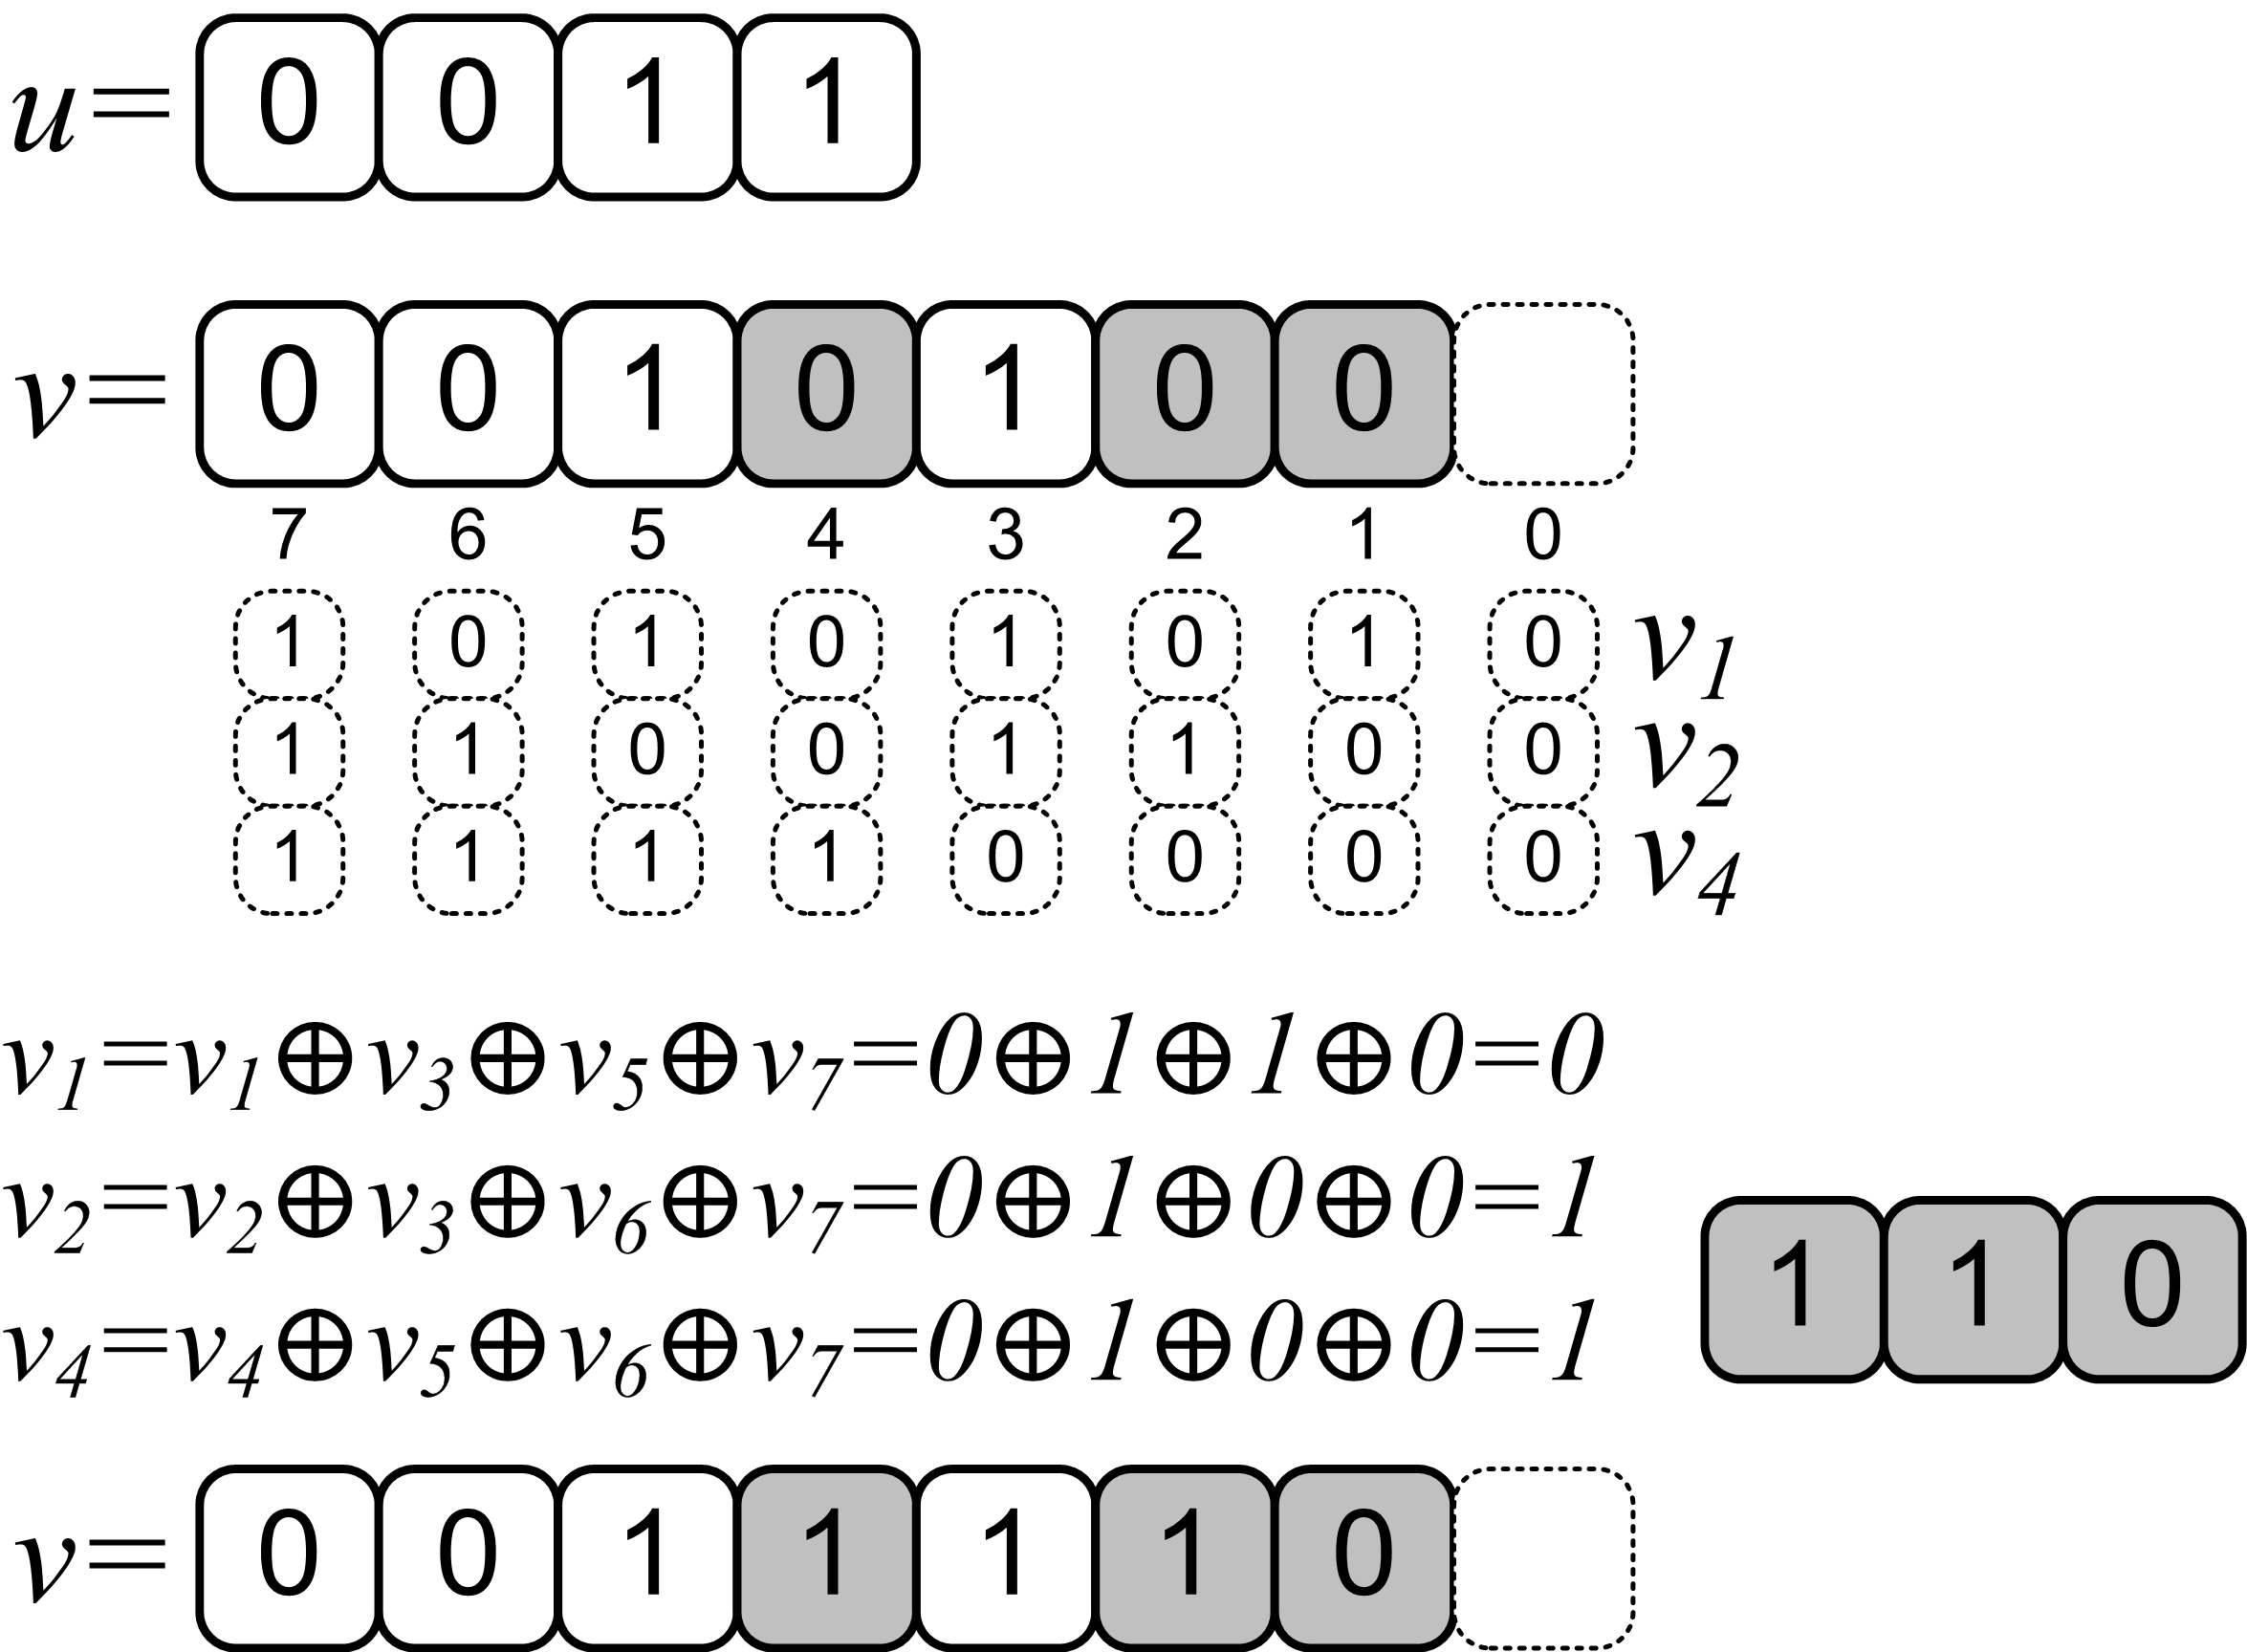
\includegraphics[width=0.6\textwidth]{fig/hammingEncode}
        \caption{Формирование код Хемминга}
        \label{fig:code:hammingEncode}
    \end{figure}
    \begin{figure}
        \centering
        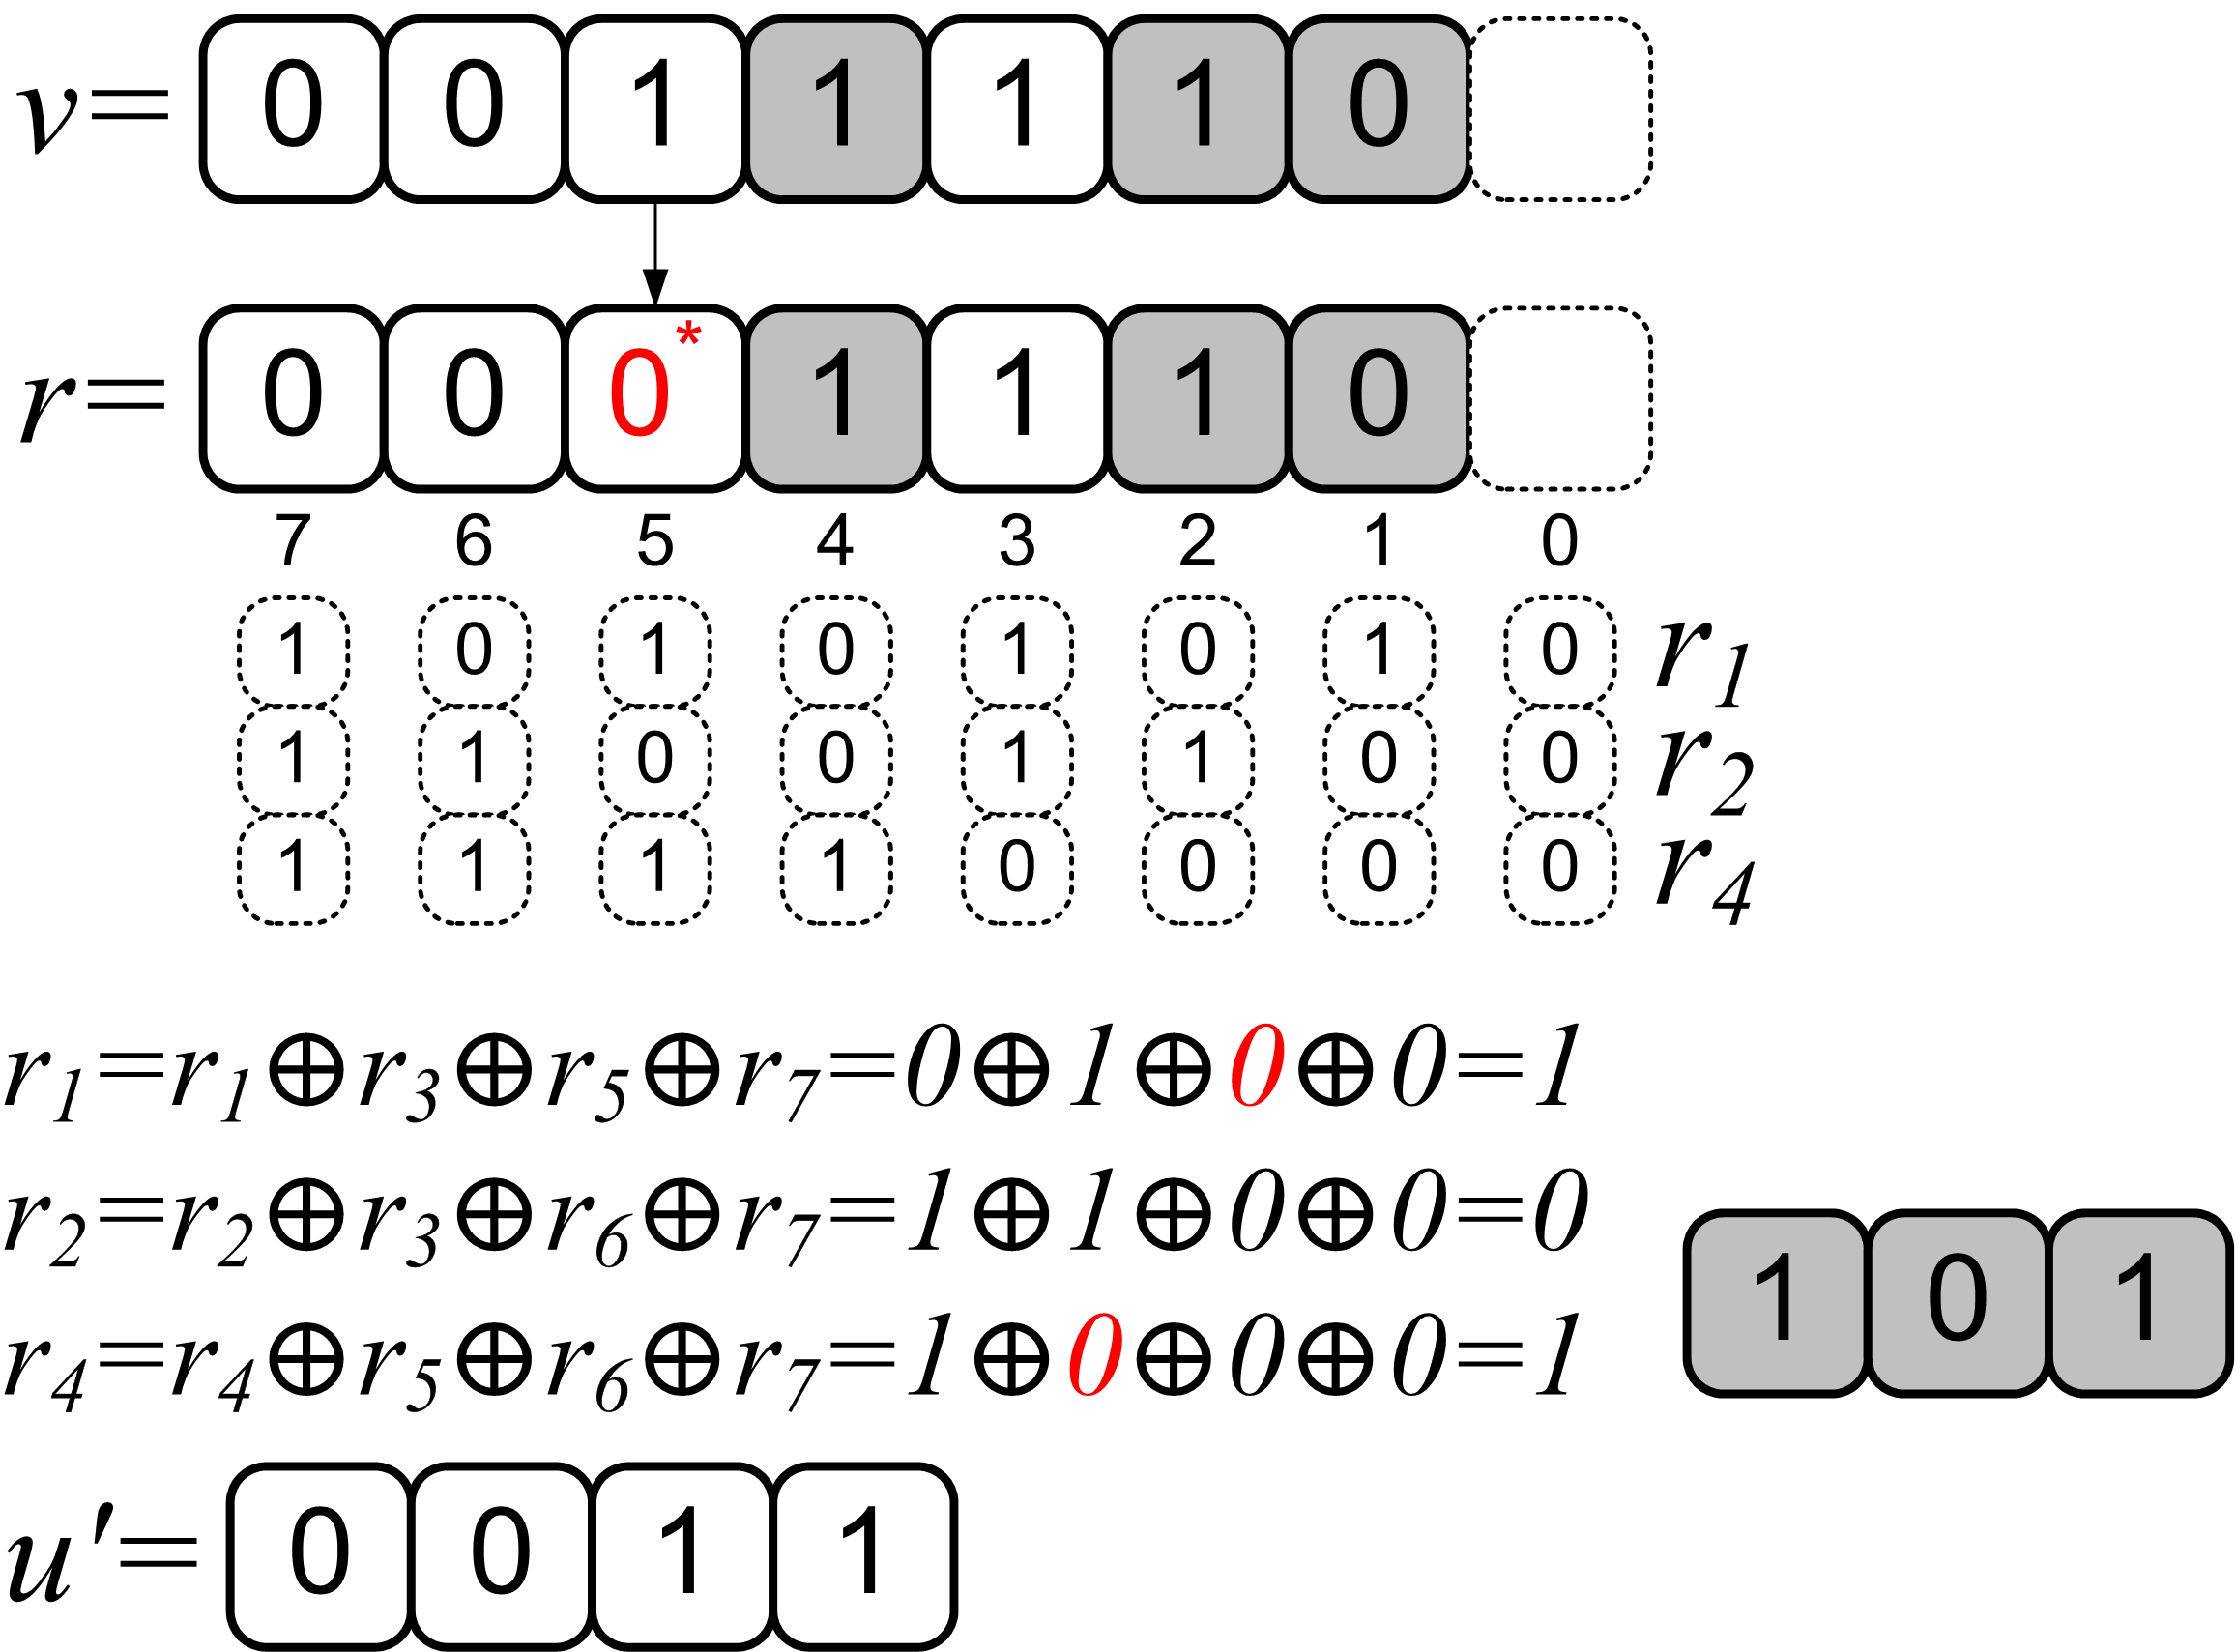
\includegraphics[width=0.6\textwidth]{fig/hammingDecode}
        \caption{Коррекция ошибки в коде Хемминга}
        \label{fig:code:hammingDecode}
    \end{figure}
    
    В результате получается код $v$. В ходе передачи происходит ошибка: пятый бит инвертируется, и пользователь принимает код $r$. Декодирование представлено на рисунке \ref{fig:code:hammingDecode}. В результате в контрольных разрядах формируется номер ошибочного бита, который инвертируется и извлекается исходный код $u'$. Код корректно исправляет одиночные ошибки и обнаруживает двойные, но может не обнаружить ошибки большей кратности.
\end{proof}


\section*{Задания}
\addcontentsline{toc}{section}{Задания}

\begin{enumerate}

    \item Множество кодовых символов $A=\{0,1\}$. Является ли приведенное ниже кодирование однозначным? Взаимно однозначным? Возможно ли декодирование? Код является префиксным? Разделима ли схема? Приведите контрпримеры, если необходимо.
    \begin{enumerate}
        \item $S=\{A,B,C,D\}$, $\delta=\{ A\mapsto 0,B\mapsto 11,C\mapsto 101, D\mapsto 110\}$;
        \item $S=\{A,B\}$, $\delta=\{ A\mapsto 0,B\mapsto 01\}$;
        \item $S=\{A,B,C\}$, $\delta=\{ A\mapsto 0,B\mapsto 01,C\mapsto 11\}$;
        \item $S=\{A,B,C,D\}$, $\delta=\{ A\mapsto 1,B\mapsto 01,C\mapsto 001,D\mapsto 000\}$.
    \end{enumerate}
    
    \item Определите длину кодовых слов для равномерного кодирования источника битами, тритами и дитами следующего количества событий:
    \begin{enumerate}
        \item $n=28$;
        \item $n=(1100101)_2$.
        \item $n=(122)_3$;
    \end{enumerate}
    
    \item Закодируйте оптимальным образом источник сообщений, если известны вероятности появления событий на его выходе. Оцените энтропию источника сообщений и соответствующего ему источника информации. Дайте оценку экономии относительно равномерного кодирования. Также закодируйте требуемую последовательность событий. Закодируйте информацию в битах или тритах, используя алгоритм Хаффмана и алгоритм Фано
    
    \begin{enumerate}
        \item 
            \begin{tabular}{|l||c|c|c|c|c|c|c|c|}
                \hline
                $s_i$   &A      &B      &C      &D      &E      &F      &G      &H      \\ \hline
                $p_i$   &0.130  &0.130  &0.126  &0.126  &0.248  &0.120  &0.060  &0.060  \\ \hline
            \end{tabular}
            
            Последовательность событий: <<GHADEFCB>>.
        \item 
            \begin{tabular}{|l||c|c|c|c|c|c|c|}
                \hline
                $s_i$   &A      &B      &C      &D      &E      &F      &G      \\ \hline
                $p_i$   &0.25   &0.125  &0.125  &0.125  &0.125  &0.125  &0.125  \\ \hline
            \end{tabular}
            
            Последовательность событий: <<DEAFABACGA>>.
        \item 
            \begin{tabular}{|l||c|c|c|c|c|c|}
                \hline
                $s_i$   &A      &B      &C      &D      &E      &F      \\ \hline
                $p_i$   &0.25   &0.25   &0.125  &0.125  &0.125  &0.125  \\ \hline
            \end{tabular}
            
            Последовательность событий: <<BDEBABAABCBF>>.
        \item 
            \begin{tabular}{|l||c|c|c|c|c|}
                \hline
                $s_i$   &A      &B      &C      &D      &E      \\ \hline
                $p_i$   &0.25   &0.25   &0.25   &0.125  &0.125 \\ \hline
            \end{tabular}
            
            Последовательность событий: <<BCACDABE>>.
    \end{enumerate}
    
    \item Закодируйте тритами $A=\{n,0,p\}$ источник, модифицировав алгоритм Хаффмана.
    
        \begin{tabular}{|l||c|c|c|c|}
            \hline
            $s_i$   &А      &Б      &В      &Г      \\ \hline
            $p_i$   &0.5    &0.3    &0.1    &0.1    \\ \hline
        \end{tabular}
        
    Почему не проходит очевидная модификация? Как гарантировать тот факт, что в последнем склеивании будут участвовать три символа?
    
    \item От двоичного источника информации была получена следующая последовательность символов: 
    \[0110100010010101010110111001111011100101110100100110001100.\] 
    
    Об источнике информации было известно, что он отражал источник сообщений с приведенными ниже характеристиками (использовался алгоритм Хаффмана и склеиваемое сообщение с большей вероятностью отмечалось символом 0). Восстановите сообщение, составленное из событий.
    
    \begin{tabular}{|l||c|c|c|c|c|c|c|c|}
        \hline
        $s_i$   &А    &З        &Л      &Н      &О      &П      &Р      &У\\ \hline
        $p_i$   &0.6  &0.0558   &0.0442 &0.0438 &0.0562 &0.0538 &0.092  &0.0542\\ \hline
    \end{tabular}
    
    \item Дана последовательность событий: 
    \[\text{ABCBCDEEDECDDEEAEBCBFCDABDEBECE}.\] 
    Требуется передать её по цифровому каналу связи (цифровой сигнал), так чтобы нагрузка на него была минимальной. Схема кодирования приемнику не важна. Рассмотрите следующие варианты: канал передает информацию в битах, в тритах и в алфавите $A=\{0, 1, 2, 3, 4\}$. Выбор алгоритма кодирования произволен.
    
    \item Проанализируйте алгоритм Лемпела-Зива. Например, дайте ответ на вопрос: когда при добавлении пары $\langle i_\omega,a\rangle$ на этапе сжатия происходит <<сжатие>> а когда, наоборот, <<расширение>>? Приведите примеры, когда <<сжатый>> текст больше исходного.
    
    \item Выполните сжатие текста 
    \[\text{<<ABABAABAABBAAAABBABAA>>}\] с помощью алгоритма Лемпела-Зива.
    
    \item Выполните сжатие текста с помощью алгоритма Лемпела-Зива, состоящего из 
    \begin{enumerate}
        \item $19$ букв <<Я>>;
        \item $12$ цепочек <<ВЫ>>;
        \item $10$ цепочек <<ОНИ>>.
    \end{enumerate}
    
    Постарайтесь найти закономерность построения кода и оценить коэффициент сжатия в зависимости от общей длины цепочки.
    
    \item Декодируйте текст, соответствующий \emph{\textbf{в}ыделенному} фрагменту кода (код --- результат сжатия методом Лемпела-Зива):
    \begin{enumerate}
        \item 
            <0,Д>, <1,А>, <0,Ы>, <3,Л>, 
            <0,Н>, <5,Е>, <0,Е>, \emph{\textbf{<0,Ц>}, 
            <7,Р>, <7,Л>, <0,Ь>, <6,Б>, 
            <4,С>, <2,Н>, <6,М>, <8,У>} 
        \item 
            <0,У>, <0,М>, <1,С>, <0,Р>,
            \emph{\textbf{<0,А>}, <5,В>, <4,О>, <4,А>, 
            <0,П>, <7,Ш>, <0,Л>, <5,Ц>, 
            <3,И>, <2,У>}
        \item 
           <0,Н>, <0,Д>, <0,О>, <0,З>, 
           <2,О >, <0,К>, <5,Б>, \emph{\textbf{<7,Р>}, 
           <3,П>, <3,У>, <6,А>, <4,У>, <1,Е>, <8,О>}
           
        \item 
            <0,Ч>, <0,З>, <0,О>, <2,Н>, 
            \emph{\textbf{<0,Я>}, <4,А>, <0,Ю>, <1,Т>, 
            <3,Н>, <0,И>, <1,Е>, <0,Г>, <9,Е>, <6,Ю>}
           
    \end{enumerate}

    \item Скажите, является ли приведенное помехоустойчивое кодирование <<утроениями>> кодом Хемминга?
    
    \item Сформируйте код Хемминга для двоичных последовательностей заданной разрядности $n$:
    \begin{enumerate}
        \item $n=5$;
        \item $n=8$;
        \item $n=10$;
        \item $n=11$.
    \end{enumerate}
    
    \item Пользователем получен вектор $r$, причем известно, что этот вектор --- результат кодирования по Хаффману вектора $u$ разрядностью $11$ бит. Что можно сказать о том, как прошла передача?
    \begin{enumerate}
        \item $r=101110101010101$;
        \item $r=111011001110111$;
        \item $r=101110101010011$;
        \item $r=101011101011100$;
        \item $r=111000101000001$;
        \item $r=101100001010111$.
    \end{enumerate}
    
    \item В каких разрядах для приведенного примера кодирования по Хаффману должны возникнуть двойные ошибки, чтобы декодер канала <<исправил\footnote{Ошибочно, конечно}>> $3$ разряд.
    
    \item Решите задачу <<о вине>>. У патриция было $243$ бочки с вином. Этого хватало, чтобы устроить скромный банкет. Завистники подложили в одну из бочек яд. Яд действует в течении суток (то есть через $24$ часа после приема яда из бочки отравленный точно умрет). Это стало известно патрицию. У патриция имеется $5$ рабов, которыми он готов пожертвовать. До начала банкета остается чуть более двух суток\footnote{В нашем цивилизованном обществе такая постановка задачи кажется жестокой. Но историю нужно признавать, а не изменять: что было, то было. Утешиться можно тем, что ни один раб при постановке задачи не пострадал\ldots}\ldots
    
    \item Обобщите приведенную в предыдущем пункте задачу <<о вине>> для случая $m$ бочек, $n$ рабов, $k$ дней.
    
\end{enumerate}
